\documentclass{article}
\usepackage[utf8]{inputenc}
\usepackage{graphicx}
\title{Problem Set 1}
\author{Péter H. Gombos}

\begin{document}
\maketitle
\section*{Problem 1}
\begin{itemize}
\item gcc - 4.2.4
\item flex - 2.5.34
\item bison - 2.3
\end{itemize}

\section*{Problem 2}
An acceptor answers "yes" if an input to a FSM is accepted, or "no" vice verca, while a lexical analyser also creates toxens.

\section*{Problem 3}
\subsection*{a}
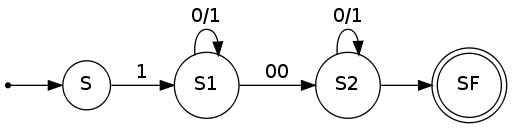
\includegraphics[scale=0.7]{nfa.png}
\subsection*{b}
The language of the automaton includes every word starting with a 1 and that contains at least two subsequent zeros.

For example,
\begin{itemize}
    \item 100
    \item 101010001100
    \item 1111100111
    \item 1000000000
\end{itemize}
\subsection*{c}
\begin{center}
\begin{tabular}{ c |  c |  c}
  \hline \hline
  STATE & 0 & 1 \\ \hline
  S & \emptyset & \{S1\}\\
  S1 & \{S1, S2\} & \{S1\} \\
  S2 & \{S2, SF\} & \{S2, SF\} \\
  SF & \emptyset & \emptyset \\
  \hline
\end{tabular}
\end{center}

\section*{Problem 4}
\begin{center}
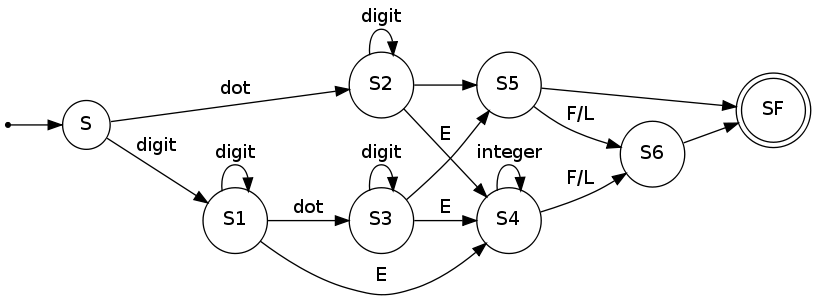
\includegraphics[scale=0.5]{nfa_float.png}
\end{center}
\end{document}
